% Options for packages loaded elsewhere
\PassOptionsToPackage{unicode}{hyperref}
\PassOptionsToPackage{hyphens}{url}
\PassOptionsToPackage{dvipsnames,svgnames,x11names}{xcolor}
%
\documentclass[
  letterpaper,
  DIV=11,
  numbers=noendperiod]{scrartcl}

\usepackage{amsmath,amssymb}
\usepackage{iftex}
\ifPDFTeX
  \usepackage[T1]{fontenc}
  \usepackage[utf8]{inputenc}
  \usepackage{textcomp} % provide euro and other symbols
\else % if luatex or xetex
  \usepackage{unicode-math}
  \defaultfontfeatures{Scale=MatchLowercase}
  \defaultfontfeatures[\rmfamily]{Ligatures=TeX,Scale=1}
\fi
\usepackage{lmodern}
\ifPDFTeX\else  
    % xetex/luatex font selection
\fi
% Use upquote if available, for straight quotes in verbatim environments
\IfFileExists{upquote.sty}{\usepackage{upquote}}{}
\IfFileExists{microtype.sty}{% use microtype if available
  \usepackage[]{microtype}
  \UseMicrotypeSet[protrusion]{basicmath} % disable protrusion for tt fonts
}{}
\makeatletter
\@ifundefined{KOMAClassName}{% if non-KOMA class
  \IfFileExists{parskip.sty}{%
    \usepackage{parskip}
  }{% else
    \setlength{\parindent}{0pt}
    \setlength{\parskip}{6pt plus 2pt minus 1pt}}
}{% if KOMA class
  \KOMAoptions{parskip=half}}
\makeatother
\usepackage{xcolor}
\setlength{\emergencystretch}{3em} % prevent overfull lines
\setcounter{secnumdepth}{5}
% Make \paragraph and \subparagraph free-standing
\ifx\paragraph\undefined\else
  \let\oldparagraph\paragraph
  \renewcommand{\paragraph}[1]{\oldparagraph{#1}\mbox{}}
\fi
\ifx\subparagraph\undefined\else
  \let\oldsubparagraph\subparagraph
  \renewcommand{\subparagraph}[1]{\oldsubparagraph{#1}\mbox{}}
\fi

\usepackage{color}
\usepackage{fancyvrb}
\newcommand{\VerbBar}{|}
\newcommand{\VERB}{\Verb[commandchars=\\\{\}]}
\DefineVerbatimEnvironment{Highlighting}{Verbatim}{commandchars=\\\{\}}
% Add ',fontsize=\small' for more characters per line
\usepackage{framed}
\definecolor{shadecolor}{RGB}{241,243,245}
\newenvironment{Shaded}{\begin{snugshade}}{\end{snugshade}}
\newcommand{\AlertTok}[1]{\textcolor[rgb]{0.68,0.00,0.00}{#1}}
\newcommand{\AnnotationTok}[1]{\textcolor[rgb]{0.37,0.37,0.37}{#1}}
\newcommand{\AttributeTok}[1]{\textcolor[rgb]{0.40,0.45,0.13}{#1}}
\newcommand{\BaseNTok}[1]{\textcolor[rgb]{0.68,0.00,0.00}{#1}}
\newcommand{\BuiltInTok}[1]{\textcolor[rgb]{0.00,0.23,0.31}{#1}}
\newcommand{\CharTok}[1]{\textcolor[rgb]{0.13,0.47,0.30}{#1}}
\newcommand{\CommentTok}[1]{\textcolor[rgb]{0.37,0.37,0.37}{#1}}
\newcommand{\CommentVarTok}[1]{\textcolor[rgb]{0.37,0.37,0.37}{\textit{#1}}}
\newcommand{\ConstantTok}[1]{\textcolor[rgb]{0.56,0.35,0.01}{#1}}
\newcommand{\ControlFlowTok}[1]{\textcolor[rgb]{0.00,0.23,0.31}{#1}}
\newcommand{\DataTypeTok}[1]{\textcolor[rgb]{0.68,0.00,0.00}{#1}}
\newcommand{\DecValTok}[1]{\textcolor[rgb]{0.68,0.00,0.00}{#1}}
\newcommand{\DocumentationTok}[1]{\textcolor[rgb]{0.37,0.37,0.37}{\textit{#1}}}
\newcommand{\ErrorTok}[1]{\textcolor[rgb]{0.68,0.00,0.00}{#1}}
\newcommand{\ExtensionTok}[1]{\textcolor[rgb]{0.00,0.23,0.31}{#1}}
\newcommand{\FloatTok}[1]{\textcolor[rgb]{0.68,0.00,0.00}{#1}}
\newcommand{\FunctionTok}[1]{\textcolor[rgb]{0.28,0.35,0.67}{#1}}
\newcommand{\ImportTok}[1]{\textcolor[rgb]{0.00,0.46,0.62}{#1}}
\newcommand{\InformationTok}[1]{\textcolor[rgb]{0.37,0.37,0.37}{#1}}
\newcommand{\KeywordTok}[1]{\textcolor[rgb]{0.00,0.23,0.31}{#1}}
\newcommand{\NormalTok}[1]{\textcolor[rgb]{0.00,0.23,0.31}{#1}}
\newcommand{\OperatorTok}[1]{\textcolor[rgb]{0.37,0.37,0.37}{#1}}
\newcommand{\OtherTok}[1]{\textcolor[rgb]{0.00,0.23,0.31}{#1}}
\newcommand{\PreprocessorTok}[1]{\textcolor[rgb]{0.68,0.00,0.00}{#1}}
\newcommand{\RegionMarkerTok}[1]{\textcolor[rgb]{0.00,0.23,0.31}{#1}}
\newcommand{\SpecialCharTok}[1]{\textcolor[rgb]{0.37,0.37,0.37}{#1}}
\newcommand{\SpecialStringTok}[1]{\textcolor[rgb]{0.13,0.47,0.30}{#1}}
\newcommand{\StringTok}[1]{\textcolor[rgb]{0.13,0.47,0.30}{#1}}
\newcommand{\VariableTok}[1]{\textcolor[rgb]{0.07,0.07,0.07}{#1}}
\newcommand{\VerbatimStringTok}[1]{\textcolor[rgb]{0.13,0.47,0.30}{#1}}
\newcommand{\WarningTok}[1]{\textcolor[rgb]{0.37,0.37,0.37}{\textit{#1}}}

\providecommand{\tightlist}{%
  \setlength{\itemsep}{0pt}\setlength{\parskip}{0pt}}\usepackage{longtable,booktabs,array}
\usepackage{calc} % for calculating minipage widths
% Correct order of tables after \paragraph or \subparagraph
\usepackage{etoolbox}
\makeatletter
\patchcmd\longtable{\par}{\if@noskipsec\mbox{}\fi\par}{}{}
\makeatother
% Allow footnotes in longtable head/foot
\IfFileExists{footnotehyper.sty}{\usepackage{footnotehyper}}{\usepackage{footnote}}
\makesavenoteenv{longtable}
\usepackage{graphicx}
\makeatletter
\def\maxwidth{\ifdim\Gin@nat@width>\linewidth\linewidth\else\Gin@nat@width\fi}
\def\maxheight{\ifdim\Gin@nat@height>\textheight\textheight\else\Gin@nat@height\fi}
\makeatother
% Scale images if necessary, so that they will not overflow the page
% margins by default, and it is still possible to overwrite the defaults
% using explicit options in \includegraphics[width, height, ...]{}
\setkeys{Gin}{width=\maxwidth,height=\maxheight,keepaspectratio}
% Set default figure placement to htbp
\makeatletter
\def\fps@figure{htbp}
\makeatother

\KOMAoption{captions}{tableheading}
\makeatletter
\@ifpackageloaded{tcolorbox}{}{\usepackage[skins,breakable]{tcolorbox}}
\@ifpackageloaded{fontawesome5}{}{\usepackage{fontawesome5}}
\definecolor{quarto-callout-color}{HTML}{909090}
\definecolor{quarto-callout-note-color}{HTML}{0758E5}
\definecolor{quarto-callout-important-color}{HTML}{CC1914}
\definecolor{quarto-callout-warning-color}{HTML}{EB9113}
\definecolor{quarto-callout-tip-color}{HTML}{00A047}
\definecolor{quarto-callout-caution-color}{HTML}{FC5300}
\definecolor{quarto-callout-color-frame}{HTML}{acacac}
\definecolor{quarto-callout-note-color-frame}{HTML}{4582ec}
\definecolor{quarto-callout-important-color-frame}{HTML}{d9534f}
\definecolor{quarto-callout-warning-color-frame}{HTML}{f0ad4e}
\definecolor{quarto-callout-tip-color-frame}{HTML}{02b875}
\definecolor{quarto-callout-caution-color-frame}{HTML}{fd7e14}
\makeatother
\makeatletter
\makeatother
\makeatletter
\makeatother
\makeatletter
\@ifpackageloaded{caption}{}{\usepackage{caption}}
\AtBeginDocument{%
\ifdefined\contentsname
  \renewcommand*\contentsname{Table of contents}
\else
  \newcommand\contentsname{Table of contents}
\fi
\ifdefined\listfigurename
  \renewcommand*\listfigurename{List of Figures}
\else
  \newcommand\listfigurename{List of Figures}
\fi
\ifdefined\listtablename
  \renewcommand*\listtablename{List of Tables}
\else
  \newcommand\listtablename{List of Tables}
\fi
\ifdefined\figurename
  \renewcommand*\figurename{Figure}
\else
  \newcommand\figurename{Figure}
\fi
\ifdefined\tablename
  \renewcommand*\tablename{Table}
\else
  \newcommand\tablename{Table}
\fi
}
\@ifpackageloaded{float}{}{\usepackage{float}}
\floatstyle{ruled}
\@ifundefined{c@chapter}{\newfloat{codelisting}{h}{lop}}{\newfloat{codelisting}{h}{lop}[chapter]}
\floatname{codelisting}{Listing}
\newcommand*\listoflistings{\listof{codelisting}{List of Listings}}
\makeatother
\makeatletter
\@ifpackageloaded{caption}{}{\usepackage{caption}}
\@ifpackageloaded{subcaption}{}{\usepackage{subcaption}}
\makeatother
\makeatletter
\@ifpackageloaded{tcolorbox}{}{\usepackage[skins,breakable]{tcolorbox}}
\makeatother
\makeatletter
\@ifundefined{shadecolor}{\definecolor{shadecolor}{rgb}{.97, .97, .97}}
\makeatother
\makeatletter
\makeatother
\makeatletter
\makeatother
\ifLuaTeX
  \usepackage{selnolig}  % disable illegal ligatures
\fi
\IfFileExists{bookmark.sty}{\usepackage{bookmark}}{\usepackage{hyperref}}
\IfFileExists{xurl.sty}{\usepackage{xurl}}{} % add URL line breaks if available
\urlstyle{same} % disable monospaced font for URLs
\hypersetup{
  pdftitle={PROJECT},
  pdfauthor={anonymous},
  colorlinks=true,
  linkcolor={blue},
  filecolor={Maroon},
  citecolor={Blue},
  urlcolor={Blue},
  pdfcreator={LaTeX via pandoc}}

\title{PROJECT}
\usepackage{etoolbox}
\makeatletter
\providecommand{\subtitle}[1]{% add subtitle to \maketitle
  \apptocmd{\@title}{\par {\large #1 \par}}{}{}
}
\makeatother
\subtitle{BLAL BLA BLA}
\author{anonymous}
\date{}

\begin{document}
\maketitle
\ifdefined\Shaded\renewenvironment{Shaded}{\begin{tcolorbox}[sharp corners, frame hidden, borderline west={3pt}{0pt}{shadecolor}, breakable, interior hidden, enhanced, boxrule=0pt]}{\end{tcolorbox}}\fi

\hypertarget{introduction}{%
\section{Introduction}\label{introduction}}

\begin{itemize}
\tightlist
\item
  Background
\item
  Problem formulation/scope
\item
  Main modeling idea
\item
  Some picture of the data?
\end{itemize}

\hypertarget{data-desctription}{%
\section{Data Desctription}\label{data-desctription}}

The ``cath'' dataset used in this report is obtained from Duke
University Cardiovascular Disease Databank. It encapsulates a collection
of 6 variables (@Data-table) that are closely related to cardiovascular
health.

\begin{longtable}[]{@{}rrrrrr@{}}
\caption{TBD }\tabularnewline
\toprule\noalign{}
sex & age & cad\_dur & choleste & sigdz & tvdlm \\
\midrule\noalign{}
\endfirsthead
\toprule\noalign{}
sex & age & cad\_dur & choleste & sigdz & tvdlm \\
\midrule\noalign{}
\endhead
\bottomrule\noalign{}
\endlastfoot
0 & 73 & 132 & 268 & 1 & 1 \\
0 & 68 & 85 & 120 & 1 & 1 \\
0 & 54 & 45 & NA & 1 & 0 \\
1 & 58 & 86 & 245 & 0 & 0 \\
1 & 56 & 7 & 269 & 0 & 0 \\
0 & 64 & 0 & NA & 1 & 0 \\
\end{longtable}

The dataset consists of four explanatory variables (\emph{sex},
\emph{age}, \emph{cad\_dur}, \emph{choleste}) and two response variables
(\emph{sigdz}, \emph{tvdlm}) that provide an overview on patient
demographics, clinical indicators, and critical outcomes related to
coronary artery disease:

\begin{itemize}
\item
  \textbf{Sex} (\emph{sex}): Categorized as 0 for male and 1 for female,
  this variable represents the gender distribution within our dataset.
\item
  \textbf{Age} (\emph{age}): Representing the age of patients in years,
  this variable serves as a demographic feature.
\item
  \textbf{Chest Pain Duration} (\emph{cad\_dur}): The duration of chest
  pain symptoms in days.
\item
  \textbf{Serum Cholesterol Level} (\emph{choleste}): Measured in
  milligrams per deciliter, serum cholesterol levels are indicative of
  lipid metabolism and play a crucial role in cardiovascular health.
\item
  \textbf{Significant Coronary Disease} (\emph{sigdz}): A binary
  variable that captures the presence (1) or absence (0) of at least
  75\% blockage in one of the major coronary arteries.
\item
  \textbf{Three Vessel Disease or Left Main Disease} (\emph{tvdlm}):
  Denoting the presence (1) or absence (0) of blockage in either all
  three coronary vessels or in the left main coronary artery.
\end{itemize}

The univariate distributions of these variables are visualized in
@Univariate-analysis.

\begin{figure}

{\centering 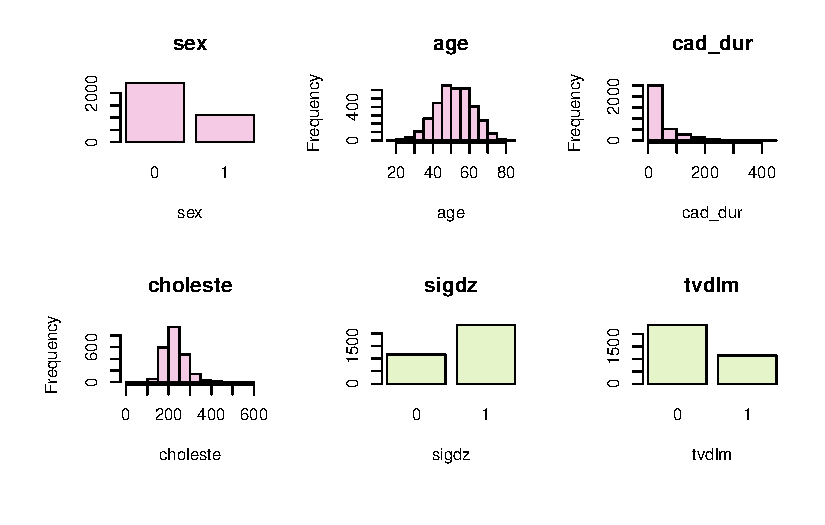
\includegraphics{project_final_files/figure-pdf/Univariate-analysis-1.pdf}

}

\caption{TBD 1}

\end{figure}

While constructing the Bayesian models to predict the probaility of
significant coronary disease, the report strives to utilize the
correlation between the explanatory variables (\emph{sex}, \emph{age},
\emph{cad\_dur}, \emph{choleste}) and the desired response variable
(\emph{sigdz}). The \emph{tvdlm} variable is not relevant in this report
as the main focus is to predict the probability of significant coronary
disease, independent of the type of the blockade.

Before the analysis, the data is preprocessed by removing \emph{tvdlm}
column and all rows that contain missing values, as well as by scaling
the continuous variables to zero mean and unit variance. After this, we
are left with \(n =\) 2258 observations. The pairwise correlations of
variables are visualized in @Bivariate-analysis. We can see that
variables \emph{sex} and \emph{age} have the most significant bivariate
correlation to the responsive variable \emph{sigdz}.

\begin{figure}

{\centering 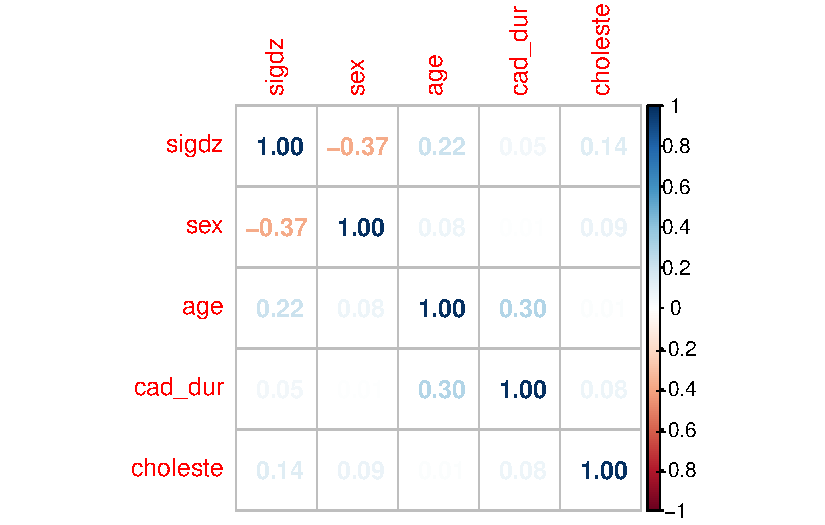
\includegraphics{project_final_files/figure-pdf/Bivariate-analysis-1.pdf}

}

\caption{TBD 3}

\end{figure}

\hypertarget{mathematical-model}{%
\section{Mathematical Model}\label{mathematical-model}}

In this analysis, we will construct two models for inferring the binary
response variable, \emph{sigdz} based on input explanatory
variables\emph{.} The first model is a generalized linear model (GLM),
namely Bayesian logistic regression. The other model is a generalized
additive mixed model (GAMM), which implements Bayesian logistic
regression with nonlinear transformations on the input variables. These
models will be referred as linear and nonlinear model, respectively.

(((To-be-done still: - Check likelihood notation for nonlinear model -
Prior justification - Check prior notations - Include priors with own
values ? - \textbf{Posteriors} ?)))

\hypertarget{the-generalized-linear-model-and-priors}{%
\subsection{The generalized linear model and
priors}\label{the-generalized-linear-model-and-priors}}

Let \(y\) be the number of times the variable \emph{sigdz} is realized
to be 1 for one individual in the dataset, and let \(x\) be the
explanatory variables for this outcome. Then, this number of successes
for one individual follows a Binomial distribution

\[
y \sim \binom{n}{y}\theta^y(1-\theta)^{n-y},
\]

where n is the number of observations for that specific individual and
\(\theta = g^{-1}(\eta)\) \((\eta = \alpha + x^{T} \beta)\) is the
probability of success (patient presenting with significant coronary
disease). The inverse link function \(g^{-1}\) maps the output of the
linear predictor \(\eta\) to a probability interval between 0 and 1.

For the binomial GLM, this project utilizes logit
\(g(x) = \ln(\frac{x}{1-x})\) as a link function, which makes it a
logistic regression model. As each individual occurs only once in the
data, \(y\) can be directly presented as the binary response variable.
Therefore, the likelihood of the response variable of one individual is
reduced to Bernoulli distribution

\[
y \sim \text{ logit}^{-1}(\eta)^y(1-\text{ logit}^{-1}(\eta))^{1-y}.
\]

The complete data likelihood is then a product of \(n =\) 2258
likelihoods, with unshared probability of success.

As in Bayesian logistic regression the scope is to infer the
distribution of the regression weights, namely the intercept \(\alpha\)
and coefficients \(\beta = [\beta_1, \beta_2, \beta_3, \beta_4]^T\), we
define the prior to be Student's \(t\)-distribution

\[
\begin{aligned} 
\alpha &\sim t_v(\mu, \sigma) \\ 
\beta_k &\sim t_v(\mu, \sigma), \ k=1,..,4 \\ 
\end{aligned} 
\]

where \(v\) is the degrees of freedom, \(\mu\) is the location and
\(\sigma\) is the scale.

The selection of prior distribution was done based on the nature of the
data. Due to correlations, there is reason to believe that the
parameters are not very close to zero, but most are still rather small
than large. Therefore, as Student's \(t\)-distribution has heavy tails
and larger scale compared to, for example, Gaussian distribution,
\(t\)-distribution is a suitable choice of prior for this purpose. The
parameters of the prior were defined to be

\[
v = 3, \quad \mu = 0, \quad \sigma = 2.5,
\]

as the coefficients can be positive or negative.

Finally, the joint posterior distribution that is simulated using
Hamiltonian Monte Carlo (HMC) is proportional to the product of
likelihood and prior distributions:

\[
p(\alpha, \beta | \bf{x}, \bf{y} ) \propto t_v(\alpha | \mu, \sigma) \times \prod^4_{k=1} t_v(\beta_k | \mu, \sigma) \times \prod^n_{i=1} \text{ logit}^{-1}(\eta_i)^{y_i}(1-\text{ logit}^{-1}(\eta_i))^{1-y_i}
\]

\hypertarget{the-generalized-additive-nonlinear-model}{%
\subsection{The generalized additive nonlinear
model}\label{the-generalized-additive-nonlinear-model}}

The additive nonlinear model on the other hand, is a generalized
additive mixed model which combines multiple functions in a way that is
not strictly linear. This allows for a more flexible relationship
between the explanatory variables and response variable \(y\). In this
report, the nonlinear model uses the same link function as the linear
model, and so the nonlinear predictor for the logistic regression model
can be written as:

\[
\text{logit} (\theta) = \eta = \alpha + \sum^4_{k=1} \beta_k f_k(x_k),
\]

where \(f_k\) are nonlinear functions that transform the explanatory
features individually. In this report, all functions of the continuous
variables are smoothing functions. The \(f_{age}\) is simply the
variable itself, due to \emph{sex} being binary variable. The smoothing
functions utilize penalized splines, allowing the model to create a
curved relationship between the features. The shape of the smoothing
functions is estimated from the data and the penalty helps avoid
overfitting. The smoothing function works by minimizing the sum of the
model fit with the smoothness / penalty (here, thin plate regression
splines (default)).

The likelihood of observation is the same as with the linear model, with
the difference that a nonlinear transformation is applied to all input
explanatory variables \(\bf{x}\). Additionally, we utilize the same
prior in both models to make them as comparable as possible. The
posterior is again similar as with the linear model, but with the
difference of nonlinear transformations on the input data.

\hypertarget{model-definitions-and-implementation}{%
\section{Model Definitions and
Implementation}\label{model-definitions-and-implementation}}

The linear and nonlinear models are implemented as Stan code with the
rstanarm package as described below. Both models were implemented with
identical number of chains, draws and warm-up. The default values
(chains = 4, draws = 4000, and warmup = 2000) were used in both cases.

\hypertarget{linear-model}{%
\subsection{Linear model}\label{linear-model}}

The linear model was implemented with the help of the \texttt{stan\_glm}
function from the rstanarm package. \texttt{stan\_glm} is used to fit
generalized linear models and performs a full Bayesian estimation with
Markov Chain Monte Carlo (MCMC) estimation instead of maximum likelihood
estimation and by adding priors to the GLM coefficients and intercept.
By defining the model parameter
\texttt{family\ =\ binomial(link\ =\ \textquotesingle{}logit\textquotesingle{})}
the model performs logistic regression.

The linear relationship between the response variable \texttt{sigdz} and
the explanatory variables are defined with the help of the
\texttt{formula} function and the prior for the regression coefficients
and intercept with the help of the \texttt{student\_t} function.

\begin{Shaded}
\begin{Highlighting}[]
\CommentTok{\# Make response variable a factor}
\NormalTok{cath}\SpecialCharTok{$}\NormalTok{sigdz }\OtherTok{\textless{}{-}} \FunctionTok{as.factor}\NormalTok{(cath}\SpecialCharTok{$}\NormalTok{sigdz)}
\NormalTok{y }\OtherTok{\textless{}{-}}\NormalTok{ cath}\SpecialCharTok{$}\NormalTok{sigdz}

\CommentTok{\# Formula}
\NormalTok{formula\_linear }\OtherTok{\textless{}{-}} \FunctionTok{formula}\NormalTok{(sigdz }\SpecialCharTok{\textasciitilde{}}\NormalTok{ sex }\SpecialCharTok{+}\NormalTok{ age }\SpecialCharTok{+}\NormalTok{ cad\_dur }\SpecialCharTok{+}\NormalTok{ choleste)}

\CommentTok{\# Prior}
\NormalTok{prior\_linear }\OtherTok{\textless{}{-}} \FunctionTok{student\_t}\NormalTok{(}\AttributeTok{df =} \DecValTok{3}\NormalTok{, }\AttributeTok{location =} \DecValTok{0}\NormalTok{, }\AttributeTok{scale =} \FloatTok{2.5}\NormalTok{)}

\CommentTok{\# The model}
\NormalTok{model\_linear }\OtherTok{\textless{}{-}} \FunctionTok{stan\_glm}\NormalTok{(formula\_linear, }\AttributeTok{data =}\NormalTok{ cath,}
                \AttributeTok{family =} \FunctionTok{binomial}\NormalTok{(}\AttributeTok{link =} \StringTok{"logit"}\NormalTok{), }
                \AttributeTok{prior =}\NormalTok{ prior\_linear, }\AttributeTok{prior\_intercept =}\NormalTok{ prior\_linear,}
                \AttributeTok{QR=}\ConstantTok{TRUE}\NormalTok{, }\AttributeTok{refresh=}\DecValTok{0}\NormalTok{)}

\CommentTok{\# saveRDS(model\_linear, file = "./additional\_files/model\_linear.rds")}
\CommentTok{\# model\_linear \textless{}{-} readRDS("./additional\_files/model\_linear.rds")                }
\end{Highlighting}
\end{Shaded}

\hypertarget{nonlinear-model}{%
\subsection{Nonlinear model}\label{nonlinear-model}}

The nonlinear model is similarly implemented utilizing
\texttt{stan\_gamm4} function from the rstanarm package and defined to
be a logistic regression model with the help of the model parameter
\texttt{family\ =\ binomial(link\ =\ \textquotesingle{}logit\textquotesingle{})}.
\texttt{stan\_gamm4} fits a generalized additive mixed model, and
performs Bayesian MCMC estimation instead of maximum likelihood
estimation. In the same way as \texttt{stan\_glm}, the model adds
independent priors to the regression coefficients and intercept.

The nonlinear relationship between the response variable \texttt{sigdz}
and the explanatory variables is again defined with the help of the
\texttt{formula} function. This time, passing the smoothing function
\texttt{s()} for all continuous explanatory variables, to allow for more
complexity in the model, while simultaneously penalizing over-fitting of
the model with the the thin plate regression splines smoothness.

The same priors are used as for the linear model for both the intercept
and the regression coefficients.

\begin{Shaded}
\begin{Highlighting}[]
\CommentTok{\# Formula}
\NormalTok{formula\_nonlinear }\OtherTok{\textless{}{-}} \FunctionTok{formula}\NormalTok{(sigdz }\SpecialCharTok{\textasciitilde{}}\NormalTok{ sex }\SpecialCharTok{+} \FunctionTok{s}\NormalTok{(age) }\SpecialCharTok{+} \FunctionTok{s}\NormalTok{(cad\_dur) }\SpecialCharTok{+} \FunctionTok{s}\NormalTok{(choleste))}

\CommentTok{\# Model definition}
\NormalTok{model\_nonlinear }\OtherTok{\textless{}{-}} \FunctionTok{stan\_gamm4}\NormalTok{(}
\NormalTok{  formula\_nonlinear, }\AttributeTok{data =}\NormalTok{ cath,}
  \AttributeTok{family =} \FunctionTok{binomial}\NormalTok{(}\AttributeTok{link =} \StringTok{"logit"}\NormalTok{),}
  \AttributeTok{prior =}\NormalTok{ prior\_linear, }\AttributeTok{prior\_intercept =}\NormalTok{ prior\_linear,}
  \AttributeTok{refresh =} \DecValTok{0}
\NormalTok{)}

\CommentTok{\# saveRDS(model\_nonlinear, file = "./additional\_files/model\_nonlinear.rds")}
\CommentTok{\# model\_nonlinear \textless{}{-} readRDS("./additional\_files/model\_nonlinear.rds")}
\end{Highlighting}
\end{Shaded}

\hypertarget{model-evaluation}{%
\section{Model Evaluation}\label{model-evaluation}}

After fitting the models, multiple evaluation metrics such as
split-\(\hat{R}\), effective sample size (ESS) and number of divergent
transitions were used to assess the convergence of MCMC chains
separately for each model. Additionally, we perform posterior predictive
checks, assess the model performances as well as compare the models
utilizing leave-one-out cross validation (LOO-CV). Finally, we perform
prior sensitivity analysis for both models.

\begin{itemize}
\tightlist
\item
  Rhat, ESS, HMC divergences, pp\_check(), loo\_compare(),
  classification accuracy
\item
  Prior sensitivity analysis
\end{itemize}

\hypertarget{convergence-diagnostics-posterior-predictive-checks}{%
\subsection{Convergence diagnostics \& posterior predictive
checks}\label{convergence-diagnostics-posterior-predictive-checks}}

For the linear model, the posterior predictive check and posterior
distributions of the parameters with 95 \% credible interval are
visualized in @linear-model-plots. As we can see, the model fits the
data relatively well, with a bit of a variation around the probability
interval endpoints.

\begin{figure}

{\centering 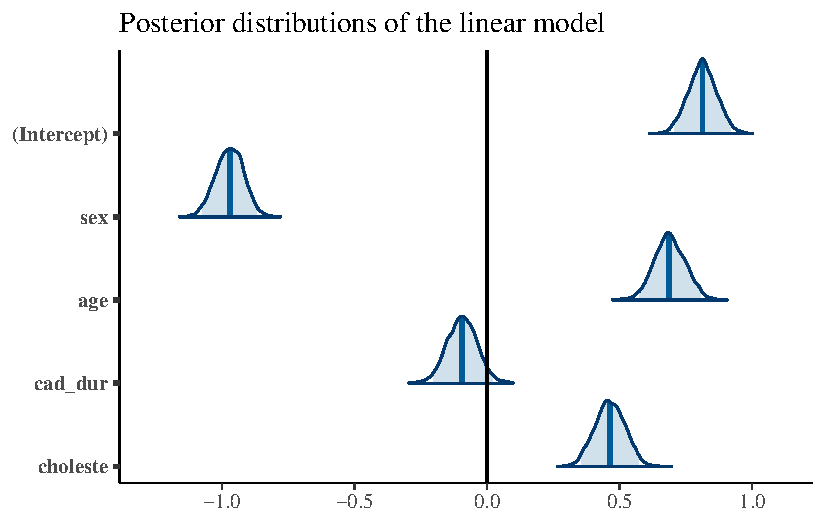
\includegraphics{project_final_files/figure-pdf/linear-model-pp-check-1.pdf}

}

\caption{TBD}

\end{figure}

\begin{figure}

{\centering 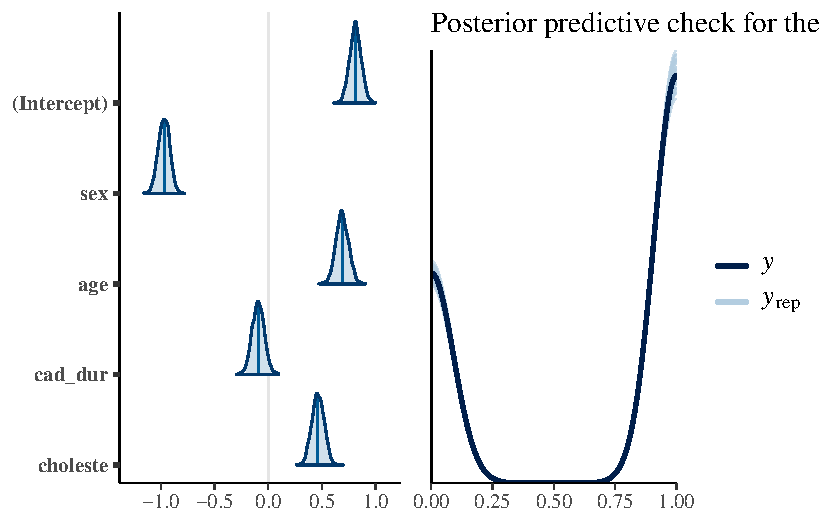
\includegraphics{project_final_files/figure-pdf/linear-model-pp-check-2.pdf}

}

\caption{TBD}

\end{figure}

The convergence diagnostics for the linear model are summarized below.

\begin{verbatim}
Split-Rhat:
\end{verbatim}

\begin{verbatim}
  (Intercept)           sex           age       cad_dur      choleste 
        1.000         1.000         0.999         0.999         1.000 
     mean_PPD log-posterior 
        1.000         1.001 
\end{verbatim}

\begin{verbatim}
Number of divergent transitions:  0 
\end{verbatim}

\begin{verbatim}
ESS ratio: 
\end{verbatim}

\begin{verbatim}
(Intercept)         sex         age     cad_dur    choleste 
    1.28925     1.13250     1.20475     1.32125     1.51725 
\end{verbatim}

\begin{verbatim}
Sd of ESS ratio:  0.145
\end{verbatim}

The HMC chains have converged, as all split-\(\hat{R}\) values are below
0.01. Additionally, there were no divergent transitions during
convergence, and thus the HMC simulation is reliable. The ratio of the
ESS to the true sample size is over 1 with all explanatory variables as
well as the intercept. Although high ESS is generally a good thing, this
also implies the MCMC samples may have a negative correlation.

For the nonlinear model, the posterior predictive check is visualized in
@nonlinear-model-pp-check. Based on visual inspection, the nonlinear
model fits the data as well as the linear model. Like with the linear
model, the posterior has a bit of a variation around the probability
interval endpoints.

\begin{figure}

{\centering 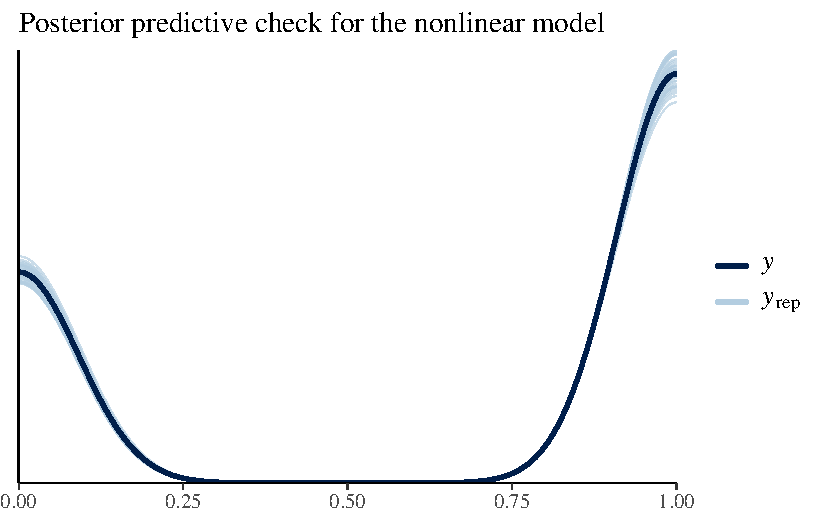
\includegraphics{project_final_files/figure-pdf/nonlinear-model-pp-check-1.pdf}

}

\caption{TBD}

\end{figure}

The convergence diagnostics for the nonlinear model are summarized
below.

\begin{Shaded}
\begin{Highlighting}[]
\NormalTok{Rhat\_nonlinear }\OtherTok{\textless{}{-}}\NormalTok{ model\_nonlinear}\SpecialCharTok{$}\NormalTok{stan\_summary[, }\StringTok{"Rhat"}\NormalTok{] }\SpecialCharTok{\%\textgreater{}\%} \FunctionTok{round}\NormalTok{(}\DecValTok{3}\NormalTok{)}
\NormalTok{np\_nonlinear }\OtherTok{\textless{}{-}} \FunctionTok{nuts\_params}\NormalTok{(model\_nonlinear)}
\NormalTok{divergents\_nonlinear }\OtherTok{\textless{}{-}} \FunctionTok{sum}\NormalTok{(}\FunctionTok{subset}\NormalTok{(np\_nonlinear, Parameter }\SpecialCharTok{==} \StringTok{"divergent\_\_"}\NormalTok{)}\SpecialCharTok{$}\NormalTok{Value)}
\NormalTok{ess\_ratio\_nonlinear }\OtherTok{\textless{}{-}} \FunctionTok{neff\_ratio}\NormalTok{(model\_nonlinear) }\SpecialCharTok{\%\textgreater{}\%} \FunctionTok{round}\NormalTok{(}\DecValTok{3}\NormalTok{)}

\NormalTok{rhat\_satisfied\_nonlinear }\OtherTok{\textless{}{-}} \FunctionTok{all}\NormalTok{(Rhat\_nonlinear }\SpecialCharTok{\textless{}=} \FloatTok{1.01}\NormalTok{)}
\NormalTok{mean\_ess\_ratio }\OtherTok{\textless{}{-}} \FunctionTok{mean}\NormalTok{(ess\_ratio\_nonlinear) }\SpecialCharTok{\%\textgreater{}\%} \FunctionTok{round}\NormalTok{(}\DecValTok{3}\NormalTok{)}
\NormalTok{sd\_ess\_ratio\_nonlinear }\OtherTok{\textless{}{-}} \FunctionTok{sd}\NormalTok{(ess\_ratio\_nonlinear) }\SpecialCharTok{\%\textgreater{}\%} \FunctionTok{round}\NormalTok{(}\DecValTok{3}\NormalTok{)}

\FunctionTok{cat}\NormalTok{(}\StringTok{"Split{-}Rhat of the first coefficients:}\SpecialCharTok{\textbackslash{}n}\StringTok{"}\NormalTok{)}
\end{Highlighting}
\end{Shaded}

\begin{verbatim}
Split-Rhat of the first coefficients:
\end{verbatim}

\begin{Shaded}
\begin{Highlighting}[]
\FunctionTok{print}\NormalTok{(}\FunctionTok{head}\NormalTok{(Rhat\_nonlinear))}
\end{Highlighting}
\end{Shaded}

\begin{verbatim}
(Intercept)         sex    s(age).1    s(age).2    s(age).3    s(age).4 
      1.000       0.999       1.000       1.000       1.001       1.001 
\end{verbatim}

\begin{Shaded}
\begin{Highlighting}[]
\FunctionTok{cat}\NormalTok{(}\StringTok{"All split{-}Rhat \textless{}= 0.01: "}\NormalTok{, rhat\_satisfied\_nonlinear, }\StringTok{"}\SpecialCharTok{\textbackslash{}n}\StringTok{"}\NormalTok{)}
\end{Highlighting}
\end{Shaded}

\begin{verbatim}
All split-Rhat <= 0.01:  TRUE 
\end{verbatim}

\begin{Shaded}
\begin{Highlighting}[]
\FunctionTok{cat}\NormalTok{(}\StringTok{"Number of divergent transitions: "}\NormalTok{,divergents\_nonlinear, }\StringTok{"}\SpecialCharTok{\textbackslash{}n}\StringTok{"}\NormalTok{)}
\end{Highlighting}
\end{Shaded}

\begin{verbatim}
Number of divergent transitions:  3 
\end{verbatim}

\begin{Shaded}
\begin{Highlighting}[]
\FunctionTok{cat}\NormalTok{(}\StringTok{"ESS ratio of the first coefficients: }\SpecialCharTok{\textbackslash{}n}\StringTok{"}\NormalTok{)}
\end{Highlighting}
\end{Shaded}

\begin{verbatim}
ESS ratio of the first coefficients: 
\end{verbatim}

\begin{Shaded}
\begin{Highlighting}[]
\FunctionTok{print}\NormalTok{(}\FunctionTok{head}\NormalTok{(ess\_ratio\_nonlinear))}
\end{Highlighting}
\end{Shaded}

\begin{verbatim}
(Intercept)         sex    s(age).1    s(age).2    s(age).3    s(age).4 
      1.464       1.453       1.085       0.773       0.396       0.818 
\end{verbatim}

\begin{Shaded}
\begin{Highlighting}[]
\FunctionTok{cat}\NormalTok{(}\StringTok{"Mean of ESS ratio: "}\NormalTok{, mean\_ess\_ratio)}
\end{Highlighting}
\end{Shaded}

\begin{verbatim}
Mean of ESS ratio:  0.819
\end{verbatim}

\begin{Shaded}
\begin{Highlighting}[]
\FunctionTok{cat}\NormalTok{(}\StringTok{"Sd of ESS ratio: "}\NormalTok{, sd\_ess\_ratio\_nonlinear)}
\end{Highlighting}
\end{Shaded}

\begin{verbatim}
Sd of ESS ratio:  0.348
\end{verbatim}

Also the MCMC chains for this model have converged, as the
split-\(\hat{R}\) is less than 0.01 for all coefficients. As with the
linear model, there were no divergent transitions during convergence,
and thus the HMC simulation is reliable. On the other hand, the ESS
ratio is on average less than 1, so a bit lower than with the linear
model. However, the standard deviation of the ESS ratios is over twice
larger than with the linear model. Low ESS ratio is not good in the
model sense, but nevertheless the nonlinear has multiple coefficients to
balance out the overall effect.

\hypertarget{model-comparison-using-loo-cv}{%
\subsection{Model comparison using
LOO-CV}\label{model-comparison-using-loo-cv}}

To compare the performance of the linear model and nonlinear model to
each other as well as to a baseline model, we will compute the expected
log-densities of the predictive distributions (ELPD) by applying Pareto
smoothed LOO-CV (PSIS-LOO) to the models. The baseline model is simply a
logistic regression model without any explanatory variables and with a
unit coefficient.

\begin{Shaded}
\begin{Highlighting}[]
\CommentTok{\# Baseline model}
\NormalTok{model\_baseline }\OtherTok{\textless{}{-}} \FunctionTok{update}\NormalTok{(model\_linear, }\AttributeTok{formula =}\NormalTok{ sigdz }\SpecialCharTok{\textasciitilde{}} \DecValTok{1}\NormalTok{, }\AttributeTok{QR =} \ConstantTok{FALSE}\NormalTok{)}
\end{Highlighting}
\end{Shaded}

The results of the PSIS-LOO for each model are presented below.

\begin{verbatim}
[1] "Linear model:"
\end{verbatim}

\begin{verbatim}

Computed from 4000 by 2258 log-likelihood matrix

         Estimate   SE
elpd_loo  -1177.6 24.4
p_loo         5.4  0.2
looic      2355.2 48.8
------
Monte Carlo SE of elpd_loo is 0.0.

All Pareto k estimates are good (k < 0.5).
See help('pareto-k-diagnostic') for details.
\end{verbatim}

\begin{verbatim}
[1] "Nonlinear model:"
\end{verbatim}

\begin{verbatim}

Computed from 4000 by 2258 log-likelihood matrix

         Estimate   SE
elpd_loo  -1170.5 24.3
p_loo        11.6  0.7
looic      2341.0 48.6
------
Monte Carlo SE of elpd_loo is 0.1.

All Pareto k estimates are good (k < 0.5).
See help('pareto-k-diagnostic') for details.
\end{verbatim}

\begin{verbatim}
[1] "Baseline model:"
\end{verbatim}

\begin{verbatim}

Computed from 4000 by 2258 log-likelihood matrix

         Estimate   SE
elpd_loo  -1448.6 15.0
p_loo         1.0  0.0
looic      2897.3 29.9
------
Monte Carlo SE of elpd_loo is 0.0.

All Pareto k estimates are good (k < 0.5).
See help('pareto-k-diagnostic') for details.
\end{verbatim}

For each model, all Pareto k estimates are \textless{} 0.5, which
implies the importance sampling gives a reliable estimate on the
computed ELPDs. Additionally, for linear and nonlinear model the p\_loo
is less than the number of parameters in the respective model, and thus
the model specifications seem to be reasonable.

To assess the model ELPDs with respect to each other, we compute the
comparison between the results of PSIS-LOO:

\begin{verbatim}
                elpd_diff se_diff
model_nonlinear    0.0       0.0 
model_linear      -7.1       3.4 
model_baseline  -278.2      21.8 
\end{verbatim}

It indeed seems that the predictive performances of both linear and
nonlinear models are better compared to the baseline model.
Additionally, the scale of the difference of standard errors (es\_diff)
of the baseline model and nonlinear model is smaller than the difference
of the ELPDs of the nonlinear and baseline model, which implies the
difference in predictive log-densities between these models is not
simply explained by the variance. Although the difference in ELPDs of
the linear and nonlinear models is small, the nonlinear model slightly
outperforms the linear model.

\hypertarget{posterior-predictive-performance-classification-accuracy}{%
\subsection{Posterior predictive performance: Classification
accuracy}\label{posterior-predictive-performance-classification-accuracy}}

To estimate the generalization error, i.e.~the generalization and
performance of models on unseen data, we compute LOO-balanced
classification accuracies for the linear and nonlinear models. The
results are summarized in @Classification-accuracies. The classification
accuracy is simply the fraction of correctly classified observations.
The balanced classification accuracy on the other hand takes into
account true positive rate (sensitivity) and true negative rate
(specificity). The latter accounts for the imbalance in our data and is
therefore more accurate estimate on the generalization error. Estimating
generalization error is highly important for practical usage of the
model, as it would be centered around predicting

\begin{longtable}[]{@{}
  >{\raggedright\arraybackslash}p{(\columnwidth - 4\tabcolsep) * \real{0.2192}}
  >{\raggedleft\arraybackslash}p{(\columnwidth - 4\tabcolsep) * \real{0.3288}}
  >{\raggedleft\arraybackslash}p{(\columnwidth - 4\tabcolsep) * \real{0.4521}}@{}}
\caption{TBD }\tabularnewline
\toprule\noalign{}
\begin{minipage}[b]{\linewidth}\raggedright
\end{minipage} & \begin{minipage}[b]{\linewidth}\raggedleft
classification\_accuracy
\end{minipage} & \begin{minipage}[b]{\linewidth}\raggedleft
balanced\_classification\_accuracy
\end{minipage} \\
\midrule\noalign{}
\endfirsthead
\toprule\noalign{}
\begin{minipage}[b]{\linewidth}\raggedright
\end{minipage} & \begin{minipage}[b]{\linewidth}\raggedleft
classification\_accuracy
\end{minipage} & \begin{minipage}[b]{\linewidth}\raggedleft
balanced\_classification\_accuracy
\end{minipage} \\
\midrule\noalign{}
\endhead
\bottomrule\noalign{}
\endlastfoot
linear\_model & 0.75 & 0.69 \\
nonlinear\_model & 0.76 & 0.69 \\
\end{longtable}

We can see that the performances of both models are nearly equal. The
classification accuracy is slightly better for the nonlinear model, but
the balanced accuracy is the same for both models. The the balanced
classification accuracy is not very high, but nevertheless, both models
outperform a random classifier.

\hypertarget{calibration-curves}{%
\subsubsection{Calibration curves}\label{calibration-curves}}

\begin{Shaded}
\begin{Highlighting}[]
\NormalTok{cplot\_linear }\OtherTok{\textless{}{-}} \FunctionTok{ggplot}\NormalTok{(}\AttributeTok{data =} \FunctionTok{data.frame}\NormalTok{(}\AttributeTok{loopred=}\NormalTok{ploo\_linear,}
  \AttributeTok{y=}\FunctionTok{as.numeric}\NormalTok{(y)}\SpecialCharTok{{-}}\DecValTok{1}\NormalTok{), }\FunctionTok{aes}\NormalTok{(}\AttributeTok{x=}\NormalTok{loopred, }\AttributeTok{y=}\NormalTok{y)) }\SpecialCharTok{+}
  \FunctionTok{stat\_smooth}\NormalTok{(}\AttributeTok{method=}\StringTok{\textquotesingle{}glm\textquotesingle{}}\NormalTok{, }\AttributeTok{formula =}\NormalTok{ y }\SpecialCharTok{\textasciitilde{}} \FunctionTok{ns}\NormalTok{(x, }\DecValTok{5}\NormalTok{), }\AttributeTok{fullrange=}\ConstantTok{TRUE}\NormalTok{, }\AttributeTok{color=}\StringTok{"deeppink"}\NormalTok{) }\SpecialCharTok{+}
  \FunctionTok{geom\_abline}\NormalTok{(}\AttributeTok{linetype =} \StringTok{\textquotesingle{}dashed\textquotesingle{}}\NormalTok{) }\SpecialCharTok{+}
  \FunctionTok{labs}\NormalTok{(}\AttributeTok{x =} \StringTok{"Predicted (LOO)"}\NormalTok{,}\AttributeTok{y =} \StringTok{"Observed"}\NormalTok{,}\AttributeTok{title =} \StringTok{"Linear model {-} Calibration plot"}\NormalTok{) }\SpecialCharTok{+}
  \FunctionTok{geom\_jitter}\NormalTok{(}\AttributeTok{height=}\FloatTok{0.02}\NormalTok{, }\AttributeTok{width=}\DecValTok{0}\NormalTok{, }\AttributeTok{alpha=}\FloatTok{0.05}\NormalTok{) }\SpecialCharTok{+}
  \FunctionTok{scale\_y\_continuous}\NormalTok{(}\AttributeTok{breaks=}\FunctionTok{seq}\NormalTok{(}\DecValTok{0}\NormalTok{,}\DecValTok{1}\NormalTok{,}\AttributeTok{by=}\FloatTok{0.1}\NormalTok{)) }\SpecialCharTok{+}
  \FunctionTok{xlim}\NormalTok{(}\FunctionTok{c}\NormalTok{(}\DecValTok{0}\NormalTok{,}\DecValTok{1}\NormalTok{)) }\SpecialCharTok{+}
  \FunctionTok{theme\_minimal}\NormalTok{()}

\NormalTok{cplot\_nonlinear }\OtherTok{\textless{}{-}} \FunctionTok{ggplot}\NormalTok{(}\AttributeTok{data =} \FunctionTok{data.frame}\NormalTok{(}\AttributeTok{loopred=}\NormalTok{ploo\_nonlinear,}
  \AttributeTok{y=}\FunctionTok{as.numeric}\NormalTok{(y)}\SpecialCharTok{{-}}\DecValTok{1}\NormalTok{), }\FunctionTok{aes}\NormalTok{(}\AttributeTok{x=}\NormalTok{loopred, }\AttributeTok{y=}\NormalTok{y)) }\SpecialCharTok{+} 
  \FunctionTok{stat\_smooth}\NormalTok{(}\AttributeTok{method=}\StringTok{\textquotesingle{}glm\textquotesingle{}}\NormalTok{, }\AttributeTok{formula =}\NormalTok{ y }\SpecialCharTok{\textasciitilde{}} \FunctionTok{ns}\NormalTok{(x, }\DecValTok{5}\NormalTok{), }\AttributeTok{fullrange=}\ConstantTok{TRUE}\NormalTok{, }\AttributeTok{color=}\StringTok{"deeppink"}\NormalTok{) }\SpecialCharTok{+}
  \FunctionTok{geom\_abline}\NormalTok{(}\AttributeTok{linetype =} \StringTok{\textquotesingle{}dashed\textquotesingle{}}\NormalTok{) }\SpecialCharTok{+} 
  \FunctionTok{labs}\NormalTok{(}\AttributeTok{x =} \StringTok{"Predicted (LOO)"}\NormalTok{,}\AttributeTok{y =} \StringTok{"Observed"}\NormalTok{,}\AttributeTok{title =} \StringTok{"Nonlinear model {-} Calibration plot"}\NormalTok{) }\SpecialCharTok{+}
  \FunctionTok{geom\_jitter}\NormalTok{(}\AttributeTok{height=}\FloatTok{0.02}\NormalTok{, }\AttributeTok{width=}\DecValTok{0}\NormalTok{, }\AttributeTok{alpha=}\FloatTok{0.05}\NormalTok{) }\SpecialCharTok{+} 
  \FunctionTok{scale\_y\_continuous}\NormalTok{(}\AttributeTok{breaks=}\FunctionTok{seq}\NormalTok{(}\DecValTok{0}\NormalTok{,}\DecValTok{1}\NormalTok{,}\AttributeTok{by=}\FloatTok{0.1}\NormalTok{)) }\SpecialCharTok{+} 
  \FunctionTok{xlim}\NormalTok{(}\FunctionTok{c}\NormalTok{(}\DecValTok{0}\NormalTok{,}\DecValTok{1}\NormalTok{)) }\SpecialCharTok{+}
  \FunctionTok{theme\_minimal}\NormalTok{() }

\FunctionTok{grid.arrange}\NormalTok{(cplot\_linear, cplot\_nonlinear, }\AttributeTok{ncol=}\DecValTok{2}\NormalTok{)}
\end{Highlighting}
\end{Shaded}

\begin{figure}[H]

{\centering 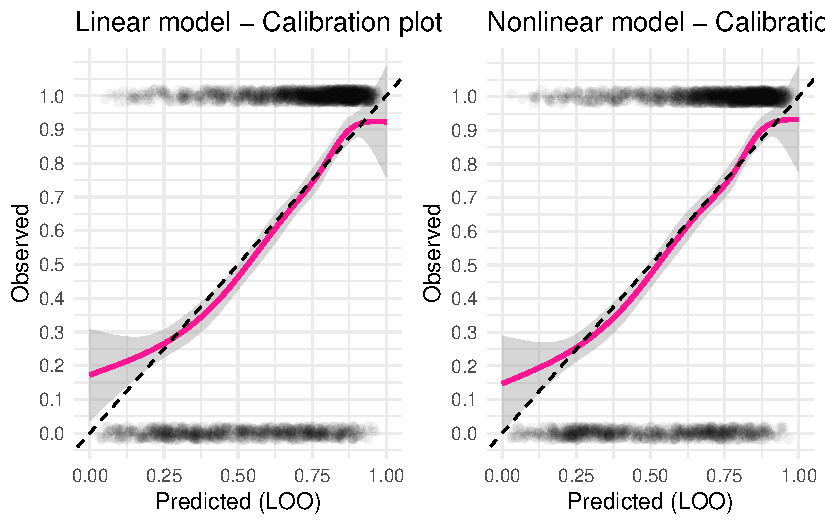
\includegraphics{project_final_files/figure-pdf/Calibration plots-1.pdf}

}

\caption{TBD X}

\end{figure}

\hypertarget{prior-sensitivity-analysis}{%
\subsection{Prior sensitivity
analysis}\label{prior-sensitivity-analysis}}

\begin{Shaded}
\begin{Highlighting}[]
\CommentTok{\#normal prior}
\NormalTok{normal\_prior }\OtherTok{\textless{}{-}} \FunctionTok{normal}\NormalTok{(}\AttributeTok{location =} \DecValTok{0}\NormalTok{, }\AttributeTok{scale =} \ConstantTok{NULL}\NormalTok{, }\AttributeTok{autoscale =} \ConstantTok{FALSE}\NormalTok{)}
\NormalTok{linear\_model\_normal\_prior }\OtherTok{\textless{}{-}} \FunctionTok{stan\_glm}\NormalTok{(formula\_linear, }\AttributeTok{data =}\NormalTok{ cath,}
                \AttributeTok{family =} \FunctionTok{binomial}\NormalTok{(}\AttributeTok{link =} \StringTok{"logit"}\NormalTok{),}
                \AttributeTok{prior =}\NormalTok{ normal\_prior, }\AttributeTok{prior\_intercept =}\NormalTok{ normal\_prior,}
                \AttributeTok{QR=}\ConstantTok{TRUE}\NormalTok{, }\AttributeTok{refresh=}\DecValTok{0}\NormalTok{)}

\CommentTok{\#default prior}
\NormalTok{linear\_model\_default\_prior }\OtherTok{\textless{}{-}} \FunctionTok{stan\_glm}\NormalTok{(formula\_linear, }\AttributeTok{data =}\NormalTok{ cath,}
                \AttributeTok{family =} \FunctionTok{binomial}\NormalTok{(}\AttributeTok{link =} \StringTok{"logit"}\NormalTok{),}
                \AttributeTok{QR=}\ConstantTok{TRUE}\NormalTok{, }\AttributeTok{refresh=}\DecValTok{0}\NormalTok{)}

\CommentTok{\#cauchy prior}
\NormalTok{cauchy\_prior }\OtherTok{\textless{}{-}} \FunctionTok{cauchy}\NormalTok{(}\AttributeTok{location =} \DecValTok{0}\NormalTok{, }\AttributeTok{scale =} \ConstantTok{NULL}\NormalTok{, }\AttributeTok{autoscale =} \ConstantTok{FALSE}\NormalTok{)}
\NormalTok{linear\_model\_cauchy\_prior }\OtherTok{\textless{}{-}} \FunctionTok{stan\_glm}\NormalTok{(formula\_linear, }\AttributeTok{data =}\NormalTok{ cath,}
                \AttributeTok{family =} \FunctionTok{binomial}\NormalTok{(}\AttributeTok{link =} \StringTok{"logit"}\NormalTok{),}
                \AttributeTok{prior =}\NormalTok{ cauchy\_prior, }\AttributeTok{prior\_intercept =}\NormalTok{ cauchy\_prior,}
                \AttributeTok{QR=}\ConstantTok{TRUE}\NormalTok{, }\AttributeTok{refresh=}\DecValTok{0}\NormalTok{)}

\CommentTok{\#normal prior, large scale N(0, 100)}
\NormalTok{normal\_prior\_sd }\OtherTok{\textless{}{-}} \FunctionTok{normal}\NormalTok{(}\DecValTok{0}\NormalTok{, }\AttributeTok{scale =} \DecValTok{100}\NormalTok{, }\AttributeTok{autoscale =} \ConstantTok{FALSE}\NormalTok{)}
\NormalTok{linear\_model\_normal\_sd }\OtherTok{\textless{}{-}} \FunctionTok{stan\_glm}\NormalTok{(formula\_linear, }\AttributeTok{data =}\NormalTok{ cath,}
                \AttributeTok{family =} \FunctionTok{binomial}\NormalTok{(}\AttributeTok{link =} \StringTok{"logit"}\NormalTok{),}
                \AttributeTok{prior =}\NormalTok{ normal\_prior\_sd, }\AttributeTok{prior\_intercept =}\NormalTok{ normal\_prior\_sd,}
                \AttributeTok{QR=}\ConstantTok{TRUE}\NormalTok{, }\AttributeTok{refresh=}\DecValTok{0}\NormalTok{)}

\CommentTok{\#normal prior, large location}
\NormalTok{normal\_prior\_loc }\OtherTok{\textless{}{-}} \FunctionTok{normal}\NormalTok{(}\DecValTok{100}\NormalTok{, }\AttributeTok{scale =} \FloatTok{2.5}\NormalTok{, }\AttributeTok{autoscale =} \ConstantTok{FALSE}\NormalTok{)}
\NormalTok{linear\_model\_normal\_loc }\OtherTok{\textless{}{-}} \FunctionTok{stan\_glm}\NormalTok{(formula\_linear, }\AttributeTok{data =}\NormalTok{ cath,}
                \AttributeTok{family =} \FunctionTok{binomial}\NormalTok{(}\AttributeTok{link =} \StringTok{"logit"}\NormalTok{),}
                \AttributeTok{prior =}\NormalTok{ normal\_prior\_loc, }\AttributeTok{prior\_intercept =}\NormalTok{ normal\_prior\_loc,}
                \AttributeTok{QR=}\ConstantTok{TRUE}\NormalTok{, }\AttributeTok{refresh=}\DecValTok{0}\NormalTok{)}

\CommentTok{\#flat prior}
\NormalTok{flat\_prior }\OtherTok{\textless{}{-}} \ConstantTok{NULL}
\NormalTok{linear\_model\_normal\_loc }\OtherTok{\textless{}{-}} \FunctionTok{stan\_glm}\NormalTok{(formula\_linear, }\AttributeTok{data =}\NormalTok{ cath,}
                \AttributeTok{family =} \FunctionTok{binomial}\NormalTok{(}\AttributeTok{link =} \StringTok{"logit"}\NormalTok{),}
                \AttributeTok{prior =}\NormalTok{ flat\_prior,}
                \AttributeTok{QR=}\ConstantTok{TRUE}\NormalTok{, }\AttributeTok{refresh=}\DecValTok{0}\NormalTok{)}
\end{Highlighting}
\end{Shaded}

Plotting the posterior distribution for each prior:

\begin{Shaded}
\begin{Highlighting}[]
\NormalTok{pplot\_normal }\OtherTok{\textless{}{-}} \FunctionTok{plot}\NormalTok{(linear\_model\_normal\_prior, }\StringTok{"areas"}\NormalTok{, }\AttributeTok{prob =} \FloatTok{0.95}\NormalTok{, }\AttributeTok{prob\_outer =} \DecValTok{1}\NormalTok{) }\SpecialCharTok{+}
  \FunctionTok{geom\_vline}\NormalTok{(}\AttributeTok{xintercept =} \DecValTok{0}\NormalTok{) }\SpecialCharTok{+} \FunctionTok{labs}\NormalTok{(}\AttributeTok{title =} \StringTok{"Normal prior"}\NormalTok{)}

\NormalTok{pplot\_default }\OtherTok{\textless{}{-}} \FunctionTok{plot}\NormalTok{(linear\_model\_default\_prior, }\StringTok{"areas"}\NormalTok{, }\AttributeTok{prob =} \FloatTok{0.95}\NormalTok{, }\AttributeTok{prob\_outer =} \DecValTok{1}\NormalTok{) }\SpecialCharTok{+}
  \FunctionTok{geom\_vline}\NormalTok{(}\AttributeTok{xintercept =} \DecValTok{0}\NormalTok{) }\SpecialCharTok{+} \FunctionTok{labs}\NormalTok{(}\AttributeTok{title =} \StringTok{"Default prior"}\NormalTok{)}

\NormalTok{pplot\_cauchy }\OtherTok{\textless{}{-}} \FunctionTok{plot}\NormalTok{(linear\_model\_cauchy\_prior, }\StringTok{"areas"}\NormalTok{, }\AttributeTok{prob =} \FloatTok{0.95}\NormalTok{, }\AttributeTok{prob\_outer =} \DecValTok{1}\NormalTok{) }\SpecialCharTok{+}
  \FunctionTok{geom\_vline}\NormalTok{(}\AttributeTok{xintercept =} \DecValTok{0}\NormalTok{) }\SpecialCharTok{+} \FunctionTok{labs}\NormalTok{(}\AttributeTok{title =} \StringTok{"Cauchy prior"}\NormalTok{)}

\NormalTok{pplot\_linear }\OtherTok{\textless{}{-}}\NormalTok{ pplot\_linear }\SpecialCharTok{+} \FunctionTok{geom\_vline}\NormalTok{(}\AttributeTok{xintercept =} \DecValTok{0}\NormalTok{) }\SpecialCharTok{+} \FunctionTok{labs}\NormalTok{(}\AttributeTok{title =} \StringTok{"Model prior"}\NormalTok{)}

\NormalTok{pplot\_normal\_sd }\OtherTok{\textless{}{-}} \FunctionTok{plot}\NormalTok{(linear\_model\_normal\_sd, }\StringTok{"areas"}\NormalTok{, }\AttributeTok{prob =} \FloatTok{0.95}\NormalTok{, }\AttributeTok{prob\_outer =} \DecValTok{1}\NormalTok{) }\SpecialCharTok{+} 
  \FunctionTok{geom\_vline}\NormalTok{(}\AttributeTok{xintercept =} \DecValTok{0}\NormalTok{) }\SpecialCharTok{+} \FunctionTok{labs}\NormalTok{(}\AttributeTok{title =} \StringTok{"N(0, 100)"}\NormalTok{)}

\NormalTok{pplot\_normal\_loc }\OtherTok{\textless{}{-}} \FunctionTok{plot}\NormalTok{(linear\_model\_normal\_loc, }\StringTok{"areas"}\NormalTok{, }\AttributeTok{prob =} \FloatTok{0.95}\NormalTok{, }\AttributeTok{prob\_outer =} \DecValTok{1}\NormalTok{) }\SpecialCharTok{+} 
  \FunctionTok{geom\_vline}\NormalTok{(}\AttributeTok{xintercept =} \DecValTok{0}\NormalTok{) }\SpecialCharTok{+} \FunctionTok{labs}\NormalTok{(}\AttributeTok{title =} \StringTok{"N(100, 0)"}\NormalTok{)}

\CommentTok{\# pplot\_flat \textless{}{-} plot(linear\_model\_flat\_prior, "areas", prob = 0.95, prob\_outer = 1) + }
  \CommentTok{\# geom\_vline(xintercept = 0) + labs(title = "flat prior")}
\CommentTok{\# , pplot\_flat}
\CommentTok{\#put desired priors into here}
\FunctionTok{grid.arrange}\NormalTok{(pplot\_normal\_sd, pplot\_normal\_loc, pplot\_default, }\AttributeTok{ncol=}\DecValTok{2}\NormalTok{, }\AttributeTok{nrow =} \DecValTok{2}\NormalTok{) }
\end{Highlighting}
\end{Shaded}

\begin{figure}[H]

{\centering 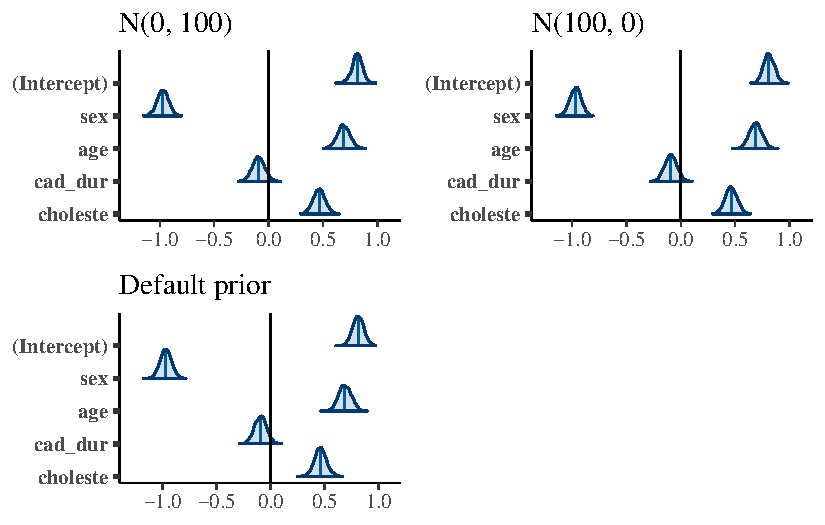
\includegraphics{project_final_files/figure-pdf/unnamed-chunk-22-1.pdf}

}

\end{figure}

\begin{Shaded}
\begin{Highlighting}[]
\CommentTok{\#normal prior}
\NormalTok{nonlinear\_model\_normal\_prior }\OtherTok{\textless{}{-}} \FunctionTok{stan\_gamm4}\NormalTok{(}
\NormalTok{  formula\_nonlinear, }\AttributeTok{data =}\NormalTok{ cath,}
  \AttributeTok{family =} \FunctionTok{binomial}\NormalTok{(}\AttributeTok{link =} \StringTok{"logit"}\NormalTok{),}
  \AttributeTok{prior =}\NormalTok{ normal\_prior, }\AttributeTok{prior\_intercept =}\NormalTok{ normal\_prior,}
  \AttributeTok{refresh =} \DecValTok{0}
\NormalTok{)}
\end{Highlighting}
\end{Shaded}

\begin{verbatim}
Warning: There were 3 divergent transitions after warmup. See
https://mc-stan.org/misc/warnings.html#divergent-transitions-after-warmup
to find out why this is a problem and how to eliminate them.
\end{verbatim}

\begin{verbatim}
Warning: Examine the pairs() plot to diagnose sampling problems
\end{verbatim}

\begin{Shaded}
\begin{Highlighting}[]
\CommentTok{\#default prior}
\NormalTok{nonlinear\_model\_default\_prior }\OtherTok{\textless{}{-}} \FunctionTok{stan\_gamm4}\NormalTok{(}
\NormalTok{  formula\_nonlinear, }\AttributeTok{data =}\NormalTok{ cath,}
  \AttributeTok{family =} \FunctionTok{binomial}\NormalTok{(}\AttributeTok{link =} \StringTok{"logit"}\NormalTok{),}
  \AttributeTok{refresh =} \DecValTok{0}
\NormalTok{)}

\CommentTok{\#cauchy prior}
\NormalTok{nonlinear\_model\_cauchy\_prior }\OtherTok{\textless{}{-}} \FunctionTok{stan\_gamm4}\NormalTok{(}
\NormalTok{  formula\_nonlinear, }\AttributeTok{data =}\NormalTok{ cath,}
  \AttributeTok{family =} \FunctionTok{binomial}\NormalTok{(}\AttributeTok{link =} \StringTok{"logit"}\NormalTok{),}
  \AttributeTok{prior =}\NormalTok{ cauchy\_prior, }\AttributeTok{prior\_intercept =}\NormalTok{ cauchy\_prior,}
  \AttributeTok{refresh =} \DecValTok{0}
\NormalTok{)}
\end{Highlighting}
\end{Shaded}

\begin{verbatim}
Warning: There were 2 divergent transitions after warmup. See
https://mc-stan.org/misc/warnings.html#divergent-transitions-after-warmup
to find out why this is a problem and how to eliminate them.

Warning: Examine the pairs() plot to diagnose sampling problems
\end{verbatim}

\begin{Shaded}
\begin{Highlighting}[]
\NormalTok{nonlinear\_pplot\_normal }\OtherTok{\textless{}{-}} \FunctionTok{plot}\NormalTok{(nonlinear\_model\_normal\_prior, }\StringTok{"areas"}\NormalTok{, }\AttributeTok{prob =} \FloatTok{0.95}\NormalTok{, }\AttributeTok{prob\_outer =} \DecValTok{1}\NormalTok{) }\SpecialCharTok{+}
  \FunctionTok{geom\_vline}\NormalTok{(}\AttributeTok{xintercept =} \DecValTok{0}\NormalTok{) }\SpecialCharTok{+} \FunctionTok{labs}\NormalTok{(}\AttributeTok{title =} \StringTok{"Normal prior"}\NormalTok{)}

\NormalTok{nonlinear\_pplot\_default }\OtherTok{\textless{}{-}} \FunctionTok{plot}\NormalTok{(nonlinear\_model\_default\_prior, }\StringTok{"areas"}\NormalTok{, }\AttributeTok{prob =} \FloatTok{0.95}\NormalTok{, }\AttributeTok{prob\_outer =} \DecValTok{1}\NormalTok{) }\SpecialCharTok{+}
  \FunctionTok{geom\_vline}\NormalTok{(}\AttributeTok{xintercept =} \DecValTok{0}\NormalTok{) }\SpecialCharTok{+} \FunctionTok{labs}\NormalTok{(}\AttributeTok{title =} \StringTok{"Default prior"}\NormalTok{)}

\NormalTok{nonlinear\_pplot\_cauchy }\OtherTok{\textless{}{-}} \FunctionTok{plot}\NormalTok{(nonlinear\_model\_cauchy\_prior, }\StringTok{"areas"}\NormalTok{, }\AttributeTok{prob =} \FloatTok{0.95}\NormalTok{, }\AttributeTok{prob\_outer =} \DecValTok{1}\NormalTok{) }\SpecialCharTok{+}
  \FunctionTok{geom\_vline}\NormalTok{(}\AttributeTok{xintercept =} \DecValTok{0}\NormalTok{) }\SpecialCharTok{+} \FunctionTok{labs}\NormalTok{(}\AttributeTok{title =} \StringTok{"Cauchy prior"}\NormalTok{)}

\NormalTok{pplot\_nonlinear }\OtherTok{\textless{}{-}} \FunctionTok{plot}\NormalTok{(model\_nonlinear, }\StringTok{"areas"}\NormalTok{, }\AttributeTok{prob =} \FloatTok{0.95}\NormalTok{, }\AttributeTok{prob\_outer =} \DecValTok{1}\NormalTok{) }\SpecialCharTok{+}
\FunctionTok{geom\_vline}\NormalTok{(}\AttributeTok{xintercept =} \DecValTok{0}\NormalTok{) }\SpecialCharTok{+} \FunctionTok{labs}\NormalTok{(}\AttributeTok{title =} \StringTok{"Model prior"}\NormalTok{)}

\FunctionTok{grid.arrange}\NormalTok{(pplot\_nonlinear, nonlinear\_pplot\_normal, nonlinear\_pplot\_default, nonlinear\_pplot\_cauchy, }\AttributeTok{ncol=}\DecValTok{2}\NormalTok{, }\AttributeTok{nrow =} \DecValTok{2}\NormalTok{) }
\end{Highlighting}
\end{Shaded}

\begin{figure}[H]

{\centering 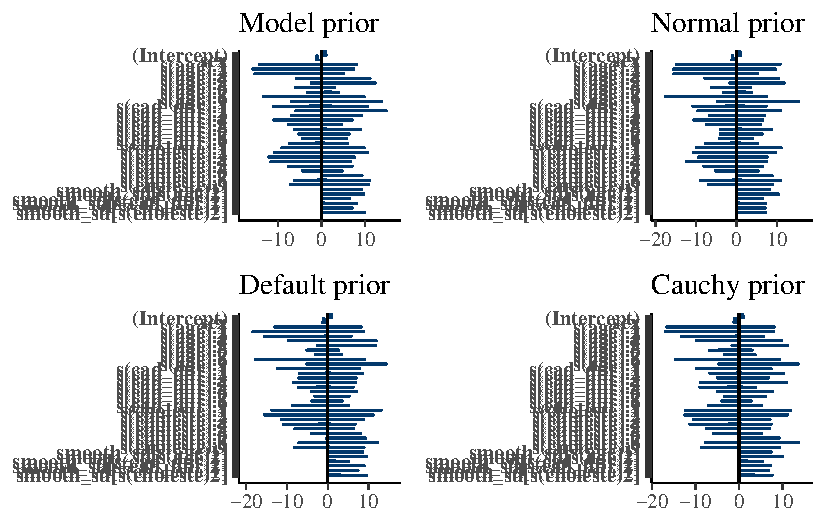
\includegraphics{project_final_files/figure-pdf/unnamed-chunk-24-1.pdf}

}

\end{figure}

\begin{Shaded}
\begin{Highlighting}[]
\NormalTok{?plot}
\end{Highlighting}
\end{Shaded}

\begin{verbatim}
starting httpd help server ... done
\end{verbatim}

\hypertarget{discussion}{%
\section{Discussion}\label{discussion}}

\begin{itemize}
\tightlist
\item
  Problems, potential improvements?
\item
  Conclusion of analysis
\end{itemize}

\hypertarget{lessons-learned}{%
\section{Lessons Learned}\label{lessons-learned}}

\hypertarget{references}{%
\section{References}\label{references}}



\end{document}
